\documentclass[stu,12pt,floatsintext]{apa7}

% ============ Required Packages ============
\usepackage[english]{babel}  % Provides language-specific definitions
\usepackage[utf8x]{inputenc}  % Allows use of non-ASCII characters
\usepackage{amsmath,amssymb}  % Advanced math formatting
\usepackage{graphicx}  % Required for inserting images
\usepackage[colorinlistoftodos]{todonotes}  % Todo notes for draft versions
\setlength{\marginparwidth}{2cm}  % Set the margin width for todo notes
\usepackage{float}        % Enhanced figure positioning
\usepackage{booktabs}     % Professional table formatting
\usepackage{hyperref}     % Better link handling
\usepackage{csquotes}     % Improved quotation management

\usepackage{microtype}  % Improves typography
\usepackage{hyperref}   % Better link and reference handling
\usepackage{csquotes}   % Improved quotation handling

\usepackage{apacite} % APA citation style
\usepackage{natbib}  % Provides citation commands
\bibliographystyle{apacite}  % APA citation style


% ============ Document Metadata ============
\title{Research Manuscript Template with Integrated Guidance}
\shorttitle{Research Writing Guide}
\author{Student Name}
\authorsaffiliations{Department of Research, University Name}
\duedate{\today}
\course{MSDS 000}
\professor{Prof. ABC} 
% ============ Abstract ============
\abstract{
    The abstract should be a single paragraph of 150-250 words.\\
  Abstract Writing Checklist:
    \begin{itemize}
        \item Include research problem/purpose
        \item Describe methodology briefly
        \item Highlight key results
        \item Emphasize conclusions and implications
    \end{itemize}
This document serves as a comprehensive template for creating APA-style manuscripts using LaTeX. It demonstrates proper formatting for various sections, including figures, tables, citations, and references. The template is compatible with APA7 styles and features extensive documentation and examples. Users can quickly adapt this template by replacing sample content with their research material while maintaining APA compliance.
}

% ============ Main Document ============
\begin{document}
\maketitle

% ============ Introduction Section ============
\section{Introduction}

\subsection{Guidance for Crafting an Effective Introduction}

\textbf{Key Components:}
\begin{itemize}
    \item Provide broad contextual background
    \item Identify the specific research problem
    \item Review relevant existing literature
    \item Highlight knowledge gaps
    \item State clear research questions/hypotheses
    \item Explain the study's significance
    \item Outline the study's structure
\end{itemize}

% Example research question formatting
\begin{quote}
\textit{Research Question: How do [specific variables] influence [outcome]?}
\end{quote}

\textbf{bold text}, 
\textit{italic text}, 
\textbf{\textit{italic and bold text}}, 
\underline{underlined text}, 
\underline{\textit{italic and underlined text}}, 
\underline{\textbf{bold and underlined text}}, 
\underline{\textbf{\textit{italic, bold, and underlined text}}}, 
\texttt{typewriter text}, 
\emph{emphasized text}, 
\textsc{small caps text}, 
{\Large large text} (e.g., large, small, tiny, etc.).


% Example of citation usage:
To cite papers, use various citation commands:
\begin{itemize}
    \item Regular citation: \cite{mujtaba2023frc}
    \item Author as part of sentence: \citet{mujtaba2024ff}
    \item Multiple citations: \citep{mujtaba2023frc, mujtaba2024ff}
\end{itemize}

% Example of research question formatting:
\begin{quote}
\textit{How do structured templates influence the quality of research manuscripts?}
\end{quote}

% ============ Methodology Section ============
\section{Methodology}
This is the methodology section that describes the approach.
\textbf{Essential Methodology Components:}
\begin{itemize}
    \item Research Design Type (Experimental, Correlational, etc.)
    \item Participant Recruitment Strategy
    \item Sample Characteristics
    \item Data Collection Instruments
    \item Procedural Details
    \item Ethical Considerations
    \item Statistical Analysis Plan
\end{itemize}

\subsection{Analysis}

% ============ Example of figure insertion ============
\begin{figure}[ht]
    \centering
    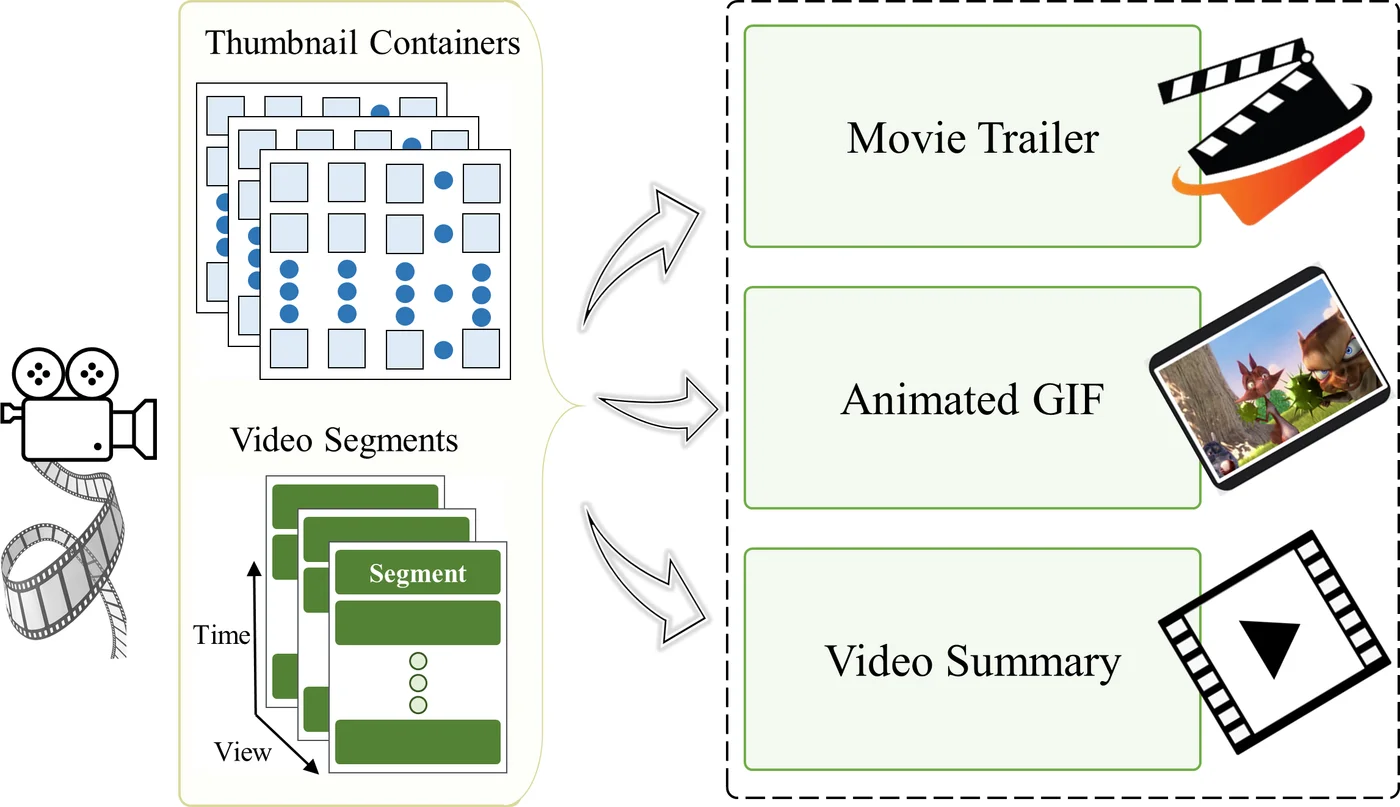
\includegraphics[width=0.75\linewidth]{figures/sample_img.png}
    \caption{Sample figure caption.}
    \label{fig:writing_scores}
\end{figure}

% ============ Example of figure insertion with scale ============
\begin{figure}[ht]
    \centering
    % Scale the image by a factor of 0.3
    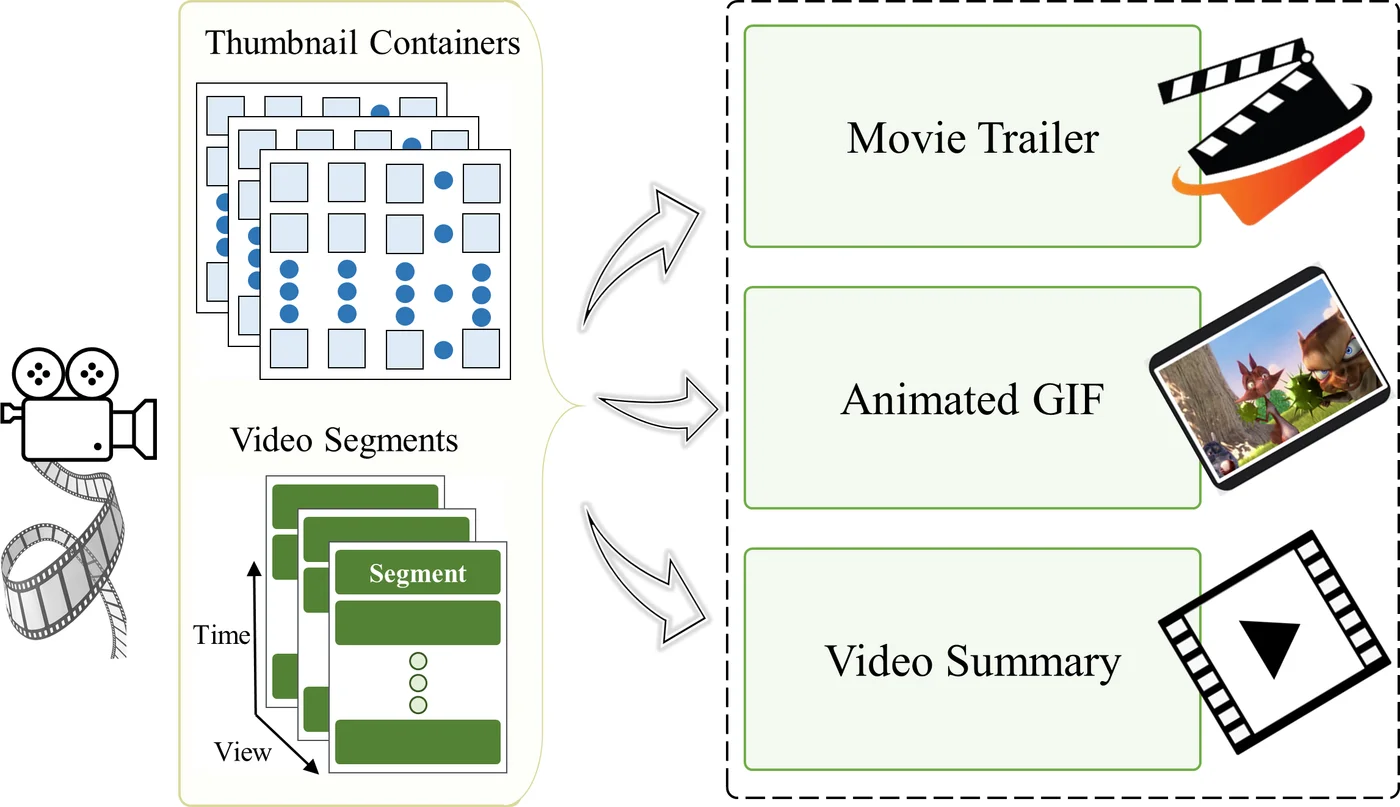
\includegraphics[scale=0.3]{figures/sample_img.png}
    \caption{Sample figure with scaling.}
    \label{fig:scaled_sample}
\end{figure}


% ============ Example of figure insertion with rotation and size ============
\begin{figure}[ht]
    \centering
    % Rotate the figure 90 degrees and set the width to 0.5 of the text width
    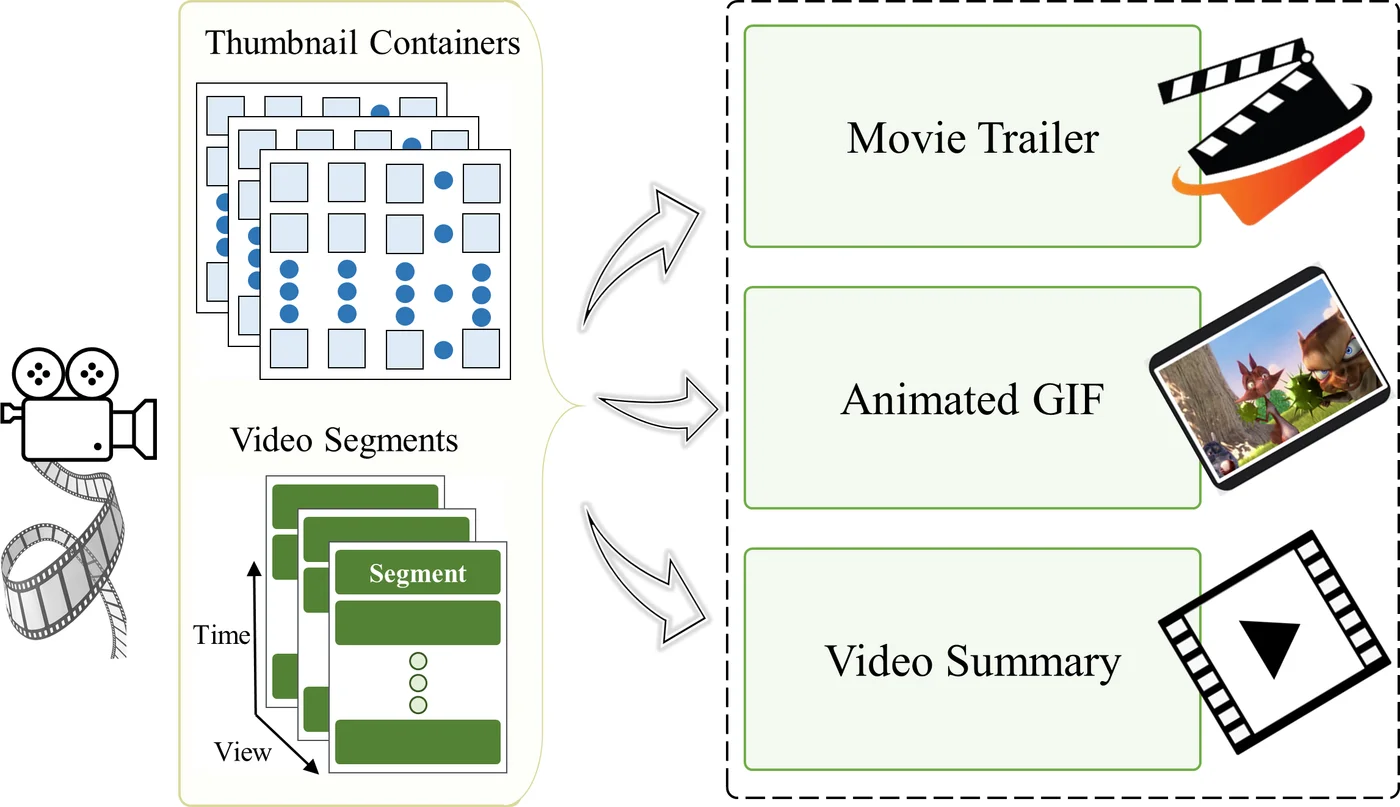
\includegraphics[angle=90, width=0.5\linewidth]{figures/sample_img.png}
    \caption{Sample figure with rotation and resized.}
    \label{fig:rotated_sample}
\end{figure}


Example of figure insertion with t, h, and !b positioning 

% ============ Example of figure insertion with t, h, and !b positioning ============
\begin{figure}[!b]
    \centering
    % Rotate the figure 90 degrees and set the width to 0.5 of the text width
    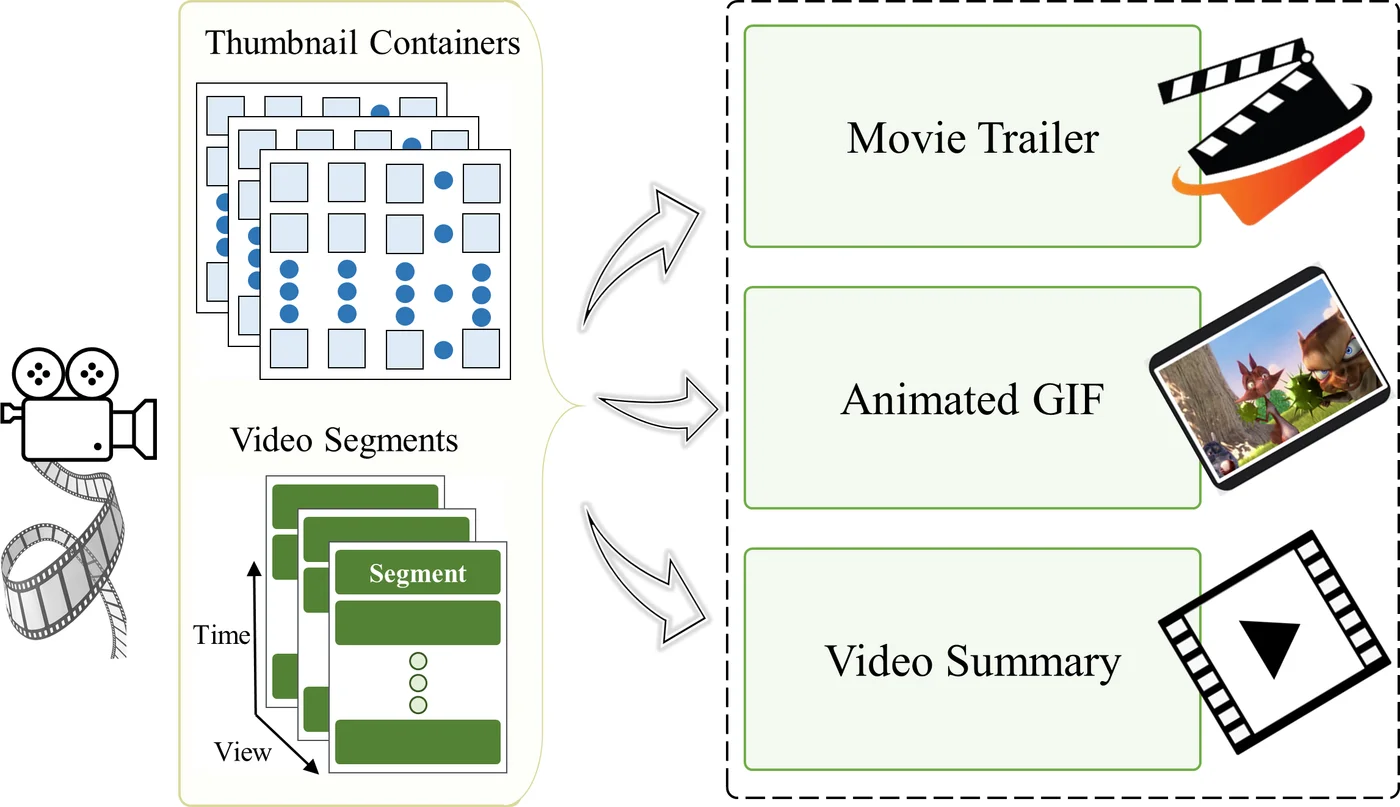
\includegraphics[angle=90, width=0.5\linewidth]{figures/sample_img.png}
    \caption{Sample figure with forced bottom placement and rotation.}
    \label{fig:sample_figre}
\end{figure}


\begin{figure}[!ht]
    \centering
    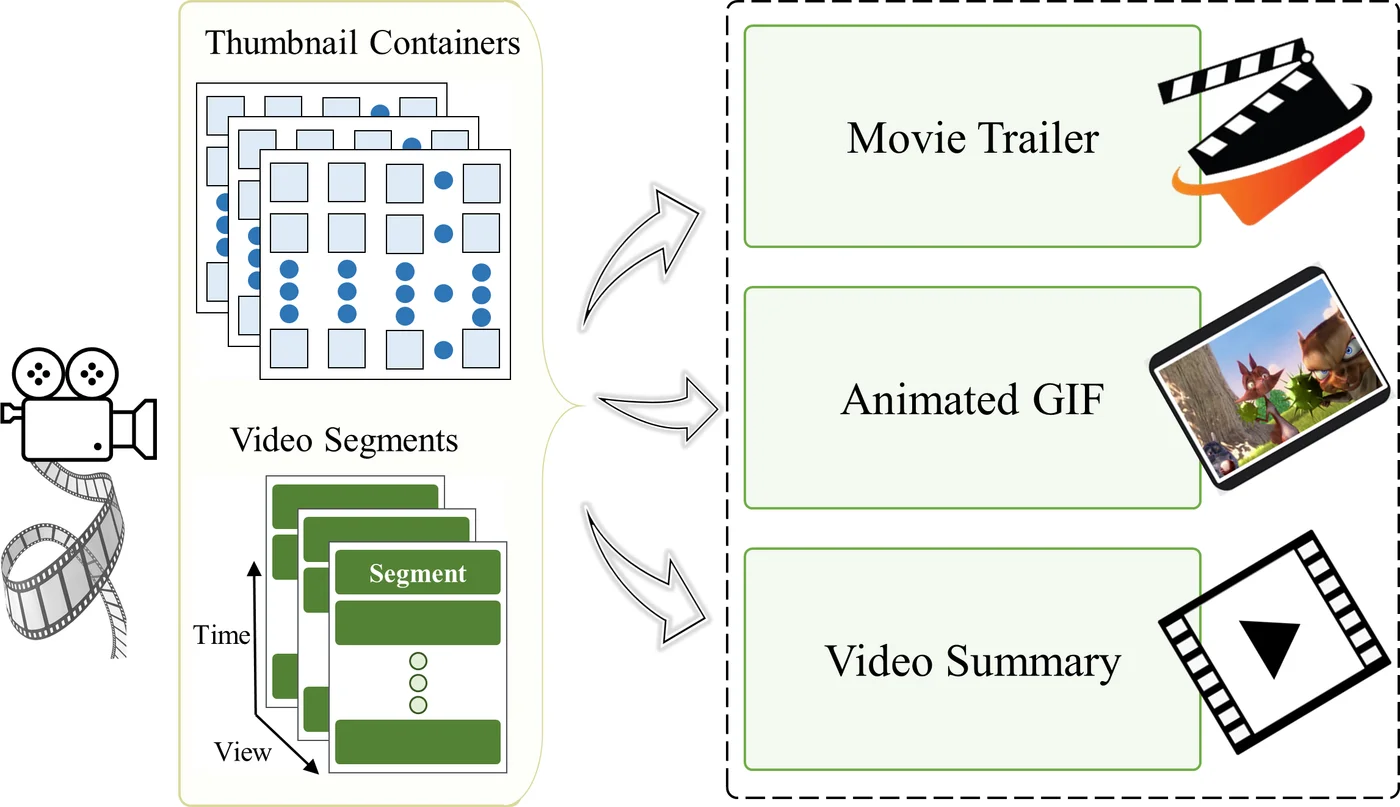
\includegraphics[width=0.6\linewidth]{figures/sample_img.png}
    \caption{Sample figure with forced placement at here or top.}
    \label{fig:sample_figure}
\end{figure}

% ============ Results Section ============
\section{Results}
\textbf{Results Presentation Strategy:}
\begin{itemize}
    \item Present data objectively
    \item Follow logical research question sequence
    \item Include descriptive and inferential statistics
    \item Utilize tables and figures effectively
    \item Report statistical significance
\end{itemize}

% Example Table
\begin{table}[ht]
    \caption{Descriptive Statistics Template}
    \centering
    \begin{tabular}{lcc}
        \hline
        Variable & Mean & Standard Deviation \\
        \hline
        Example 1 & 0.00 & 0.00 \\
        Example 2 & 0.00 & 0.00 \\
        \hline
    \end{tabular}
\end{table}

% ============ Discussion Section ============
\section{Discussion and Conclusions}
\textbf{Discussion Section Checklist:}
\begin{itemize}
    \item Summarize key findings
    \item Interpret results relative to hypotheses
    \item Compare with existing literature
    \item Acknowledge study limitations
    \item Suggest future research directions
    \item Discuss practical implications
\end{itemize}

Our results align with previous research \citep{mujtaba2023frc}. This suggests several key points:

\begin{itemize}
    \item one
    \item two
    \item three
\end{itemize}

% ============ References Section ============
\bibliography{references}

\end{document}
